%---------- Inleiding ---------------------------------------------------------

% TODO: Is dit voorstel gebaseerd op een paper van Research Methods die je
% vorig jaar hebt ingediend? Heb je daarbij eventueel samengewerkt met een
% andere student?
% Zo ja, haal dan de tekst hieronder uit commentaar en pas aan.

%\paragraph{Opmerking}

% Dit voorstel is gebaseerd op het onderzoeksvoorstel dat werd geschreven in het
% kader van het vak Research Methods dat ik (vorig/dit) academiejaar heb
% uitgewerkt (met medesturent VOORNAAM NAAM als mede-auteur).
% 

\section{Inleiding}%
\label{sec:inleiding}

Het implementeren van ETL's en ELT's speelt een kritieke rol in de development binnen Net IT. Net IT is een bedrijf gespecialiseerd in Customer Relationship Management (CRM). Een CRM-systeem is een applicatie om voeling te houden met klanten en om processen te stroomlijnen en meer winst te genereren. Doordat Net IT een Microsoft Partner is zullen ze CRM-toepassingen implementeren met Microsoft Dynamics 365 en intelligente bedrijfstoepassingen met Microsoft Power Platform. Binnen Microsoft 365 Dynamics Customer Engagement worden er CSV bestanden geëxporteerd naar Azure Data Lake. Deze data wordt minstens dagelijks opgekuist, aangevuld en opgesplitst om naar de klant te kunnen doorsturen via SFTP of e-mail. Momenteel wordt dit gedaan door ETL's en ELT's te implementeren in Azure Data Factory, gebruik makend van de UI tools die aangeboden worden. Doordat dit niet de enige mogelijkheid is om dit te implementeren zal er gekeken worden naar de verschillende opties die er zijn. Aangezien Net IT een Microsoft Partner is zal er vooral gekeken worden binnen Microsoft Azure. Deze verschillende mogelijkheden zullen vergeleken worden op basis van performantie, kostprijs (voor dezelfde performantie), complexiteit, moeilijkheidsgraad in opzet en configuratie van de resources, verschil in implementatietijd en mogelijkheden van de tool. De methode die gebruikt zal worden is een gemengde aanpak gebaseerd op literatuuronderzoek en het opstellen van proof-of-concepts voor de gegeven use case van Net IT. Dit zal resulteren in een gedetailleerd vergelijkingsrapport, inclusief aanbeveling voor de meest geschikte aanpak voor het implementeren van ETL's of ELT's voor de gegeven use case.

\section{Literatuurstudie}%
\label{sec:literatuurstudie}

Als data engineer krijgt men data in veel verschillende vormen. Het is dus noodzakelijk om deze data klaar te maken voor business analytics.~\autocite{Kromer2022} Hiervoor maakt men gebruik van ETL's en ELT's. Dit zijn processen die organisaties gebruiken voor het verzamelen en samenvoegen van data uit meerdere bronnen. Bij ETL's wordt de data getransformeerd voor het naar de doelopslagplaats geladen wordt, terwijl dit bij ELT's pas achteraf gebeurd. Daardoor staat ETL voor Extract, Transform and Load en ELT voor Extract, Load and Transform.~\autocite{Bartley2023} 

In Azure zijn er meerdere mogelijkheden voor het implementeren van ETL's en ELT's. Één van deze mogelijkheden is Azure Data Factory. Zoals te zien in de enquête van~\textcite{Sreemathy2021} is dit de meest populaire data integratie service die aangeboden wordt door de cloud providers. Binnen Azure Data Factory kan er gebruik gemaakt worden van Mapping Data Flows, dit is een codevrije manier waarmee ETL's opgebouwd kunnen worden. De logica achter de ETL kan hierna makkelijk getest worden op live data en samples.~\autocite{Kromer2022a} 

Daarnaast biedt Azure ook Azure Databricks aan. Het verschil hierbij is dat de ETL's worden geïmplementeerd via code terwijl dat bij Azure Data Factory via de UI tools kan gebeurt. Azure Databricks is gebaseerd op het Apache Spark open source project. Het grote voordeel is dat het platform het toelaat om makkelijker te kunnen samen werken. Daarnaast is Apache Spark niet enkel gelimiteerd tot het maken van ETL's maar kan het ook gebruikt worden voor real-time analytics, machine learning, graph processing, etc.~\autocite{Etaati2019}

Azure is niet de enigste cloud provider die ETL tools aanbiedt. Zo heeft AWS bijvoorbeeld AWS Glue~\autocite{Khan2024} en Google Cloud heeft Google Data Fusion.~\autocite{Jaiswal2022}

\section{Methodologie}%
\label{sec:methodologie}

\begin{center}
    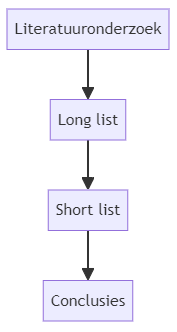
\includegraphics[width=0.2\textwidth]{../voorstel/graphics/methodologie.png}    
\end{center}

De eerste fase is het literatuuronderzoek. Hierbij wordt er gekeken naar welke mogelijkheden er zijn voor het implementeren van ETL's en ELT's. Er zal vooral gefocust worden op de mogelijkheden binnen Azure maar ook andere opties zullen bekeken worden. Dit zal gedaan worden met behulp van academische onderzoekstools zoals Google Scholar en andere relevante databanken en bronnen. Ook de documentatie van Azure, casestudies van bedrijven die gebruik maken van Azure en blogs van experts op dit vakgebied zullen hier zeker bij van pas komen. Deze fase zal ook zeker in samenwerkingen met Net IT gebeuren zodat de huidige gebruikte technologieën voor het implementeren van ETL's en ELT's zeker niet uitgesloten worden. Dit onderdeel zal naar verwachting vier weken in beslag nemen. 

In de tweede fase zullen de resultaten van het literatuuronderzoek samengevat worden in een long list. Dit onderdeel zal naar verwachting twee weken duren.

In de derde fase zullen de meest interessante opties uit de long list samengevat worden in een short list. Hierbij zal gekeken worden naar wat het interessantst is voor Net IT. Doordat dit een kleine fase is zal dit bij de tijd van de tweede fase horen.

In de vierde fase zullen er vergelijkingscriteria opgesteld worden voor de gegeven use case door Net IT. Het is belangrijk om te weten wat er moet vergeleken worden. Belangrijk om op te merken is dat niet alles even meetbaar zal zijn. Er zal dus goed gekeken worden naar hoe de vergelijkingscriteria gemeten kunnen worden. Dit onderdeel zal naar verwachting één week duren.

In de vijfde fase zal er op basis van de short list en vergelijkingscriteria een proof-of-concept uitgewerkt worden voor elke mogelijkheid dat er binnen Azure is. Er zal een situatie (gegeven door Net IT) opgezet worden met dummy data in een data lake. Het doel is dat er op basis van deze data export bestanden zullen gemaakt worden. Dit zal de langste fase zijn en zal dus vier weken in beslag nemen.

De zesde en laatste fase, die naar verwachting één week zal duren, is de evaluatie van de opties die we hebben onderzocht. Het doel is om te tonen welke optie het beste is. Daardoor zal het resultaat van deze analyse een gedetailleerd vergelijkingsrapport zijn en een aanbeveling voor welke optie het beste is.


%---------- Verwachte resultaten ----------------------------------------------
\section{Verwacht resultaat, conclusie}%
\label{sec:verwachte_resultaten}

Het resultaat zal een gedetailleerd vergelijkingsrapport zijn, inclusief aanbevelingen voor de meest geschikte aanpak voor het implementeren van ETL's of ELT's voor de gegeven use case. Daarnaast zal er ook een resultaat per vergelijkingscriteria zijn zodat Net IT zelf ook een dieper inzicht krijgt in bijvoorbeeld operationele implicaties, kostenstructuur, etc.
